%!TEX root = ttc15-train-benchmark-sigma.tex

% \vspace*{-3mm}
% \enlargethispage{7mm}

\section{Evaluation}
\label{sec:Evaluation}

In this section we provide an evaluation of our solution following the categories given by the case study.

\subsection{Correctness and Completeness of Model Queries and Transformations}

We developed a solution for all of the tasks required by the case study and the solution passes the provided tests.

\subsection{Conciseness}

The solution itself consists of 52 lines of Scala code the internal DSL developed for this case study.
The DSL itself has been implemented using 20 lines of Scala code using \SIGMA.
The integration part consists of three files with the total of 65 lines.
All measures are source lines only excluding comments and new lines.
Given these measures, we believe that the code is quite concise.

\subsection{Readability}

Next to being concise, the solution is also quite expressive.
This means that the given problem (queries and repair transformations) naturally maps into the implementation.
The higher-level abstraction provided by both \SIGMA and the internal DSLs helps to facilitate it making a significant improvement over the Java reference implementation.
% It is important to note that we could have provided even a more flexible syntax, but that would obscure the implementation of the DSL (the type definition) and make the possible error messages more cryptic.
%
Next to being concise and expressive, the code is also type-safe as Scala is statically typed language.
A notable consequence is that it is very easy to use the DSL with an IDE like Eclipse or IntelliJ that provides a robust code completing functionalities, outline views and other features increasing one's productivity.

In summary, while readability is a subjective matter and largely depends on the background and experience of users, we believe that \SIGMA scores well.
Thanks to the syntax of Scala which is close to one of Java/C++ and hence shall be familiar to many developers.
The expressiveness of the first-order logic collection operation should be familiar to anyone knowing OCL or any other function language.


\subsection{Performance on Large Models}

The tests have been performed on an 2.3 GHz Intel Core i7 machine with 16 GB of RAM being dedicated to the JVM process.
We ran our solution together with the reference implementation in Java.
We used the model instances from size 1 to 8192 and set 8GB memory to be dedicated to the JVM.
The corresponding results are shown in the figures~\ref{fig:SigmaFixedValidationBatch} and~\ref{fig:SigmaFixedReValidationBatch}.
We compare them to the Java solution which is shown in the figures~\ref{fig:JavaFixedValidationBatch} and~\ref{fig:JavaFixedReValidationBatch}.
We get a similar performance which has been expected due to the fact that Scala compiles directly to Java bytecode and we use the same underlying libraries for accessing EMF models.
This shows that we can leverage from concise and expressive queries without sacrificing performance.

It is important to note that we do not developed any extra functionality for these benchmarks---\Ie no caching or incremental validations.
On the other hand, functional approach we have selected makes it perfect for further parallelization.
Moreover, for even larger models we could easily port the solution into big data analysis platforms such as Hadoop\footnote{\url{https://hadoop.apache.org/}}.
This would be rather difficult given the imperative Java implementation.

\begin{figure}[h!tb]
  \centering
  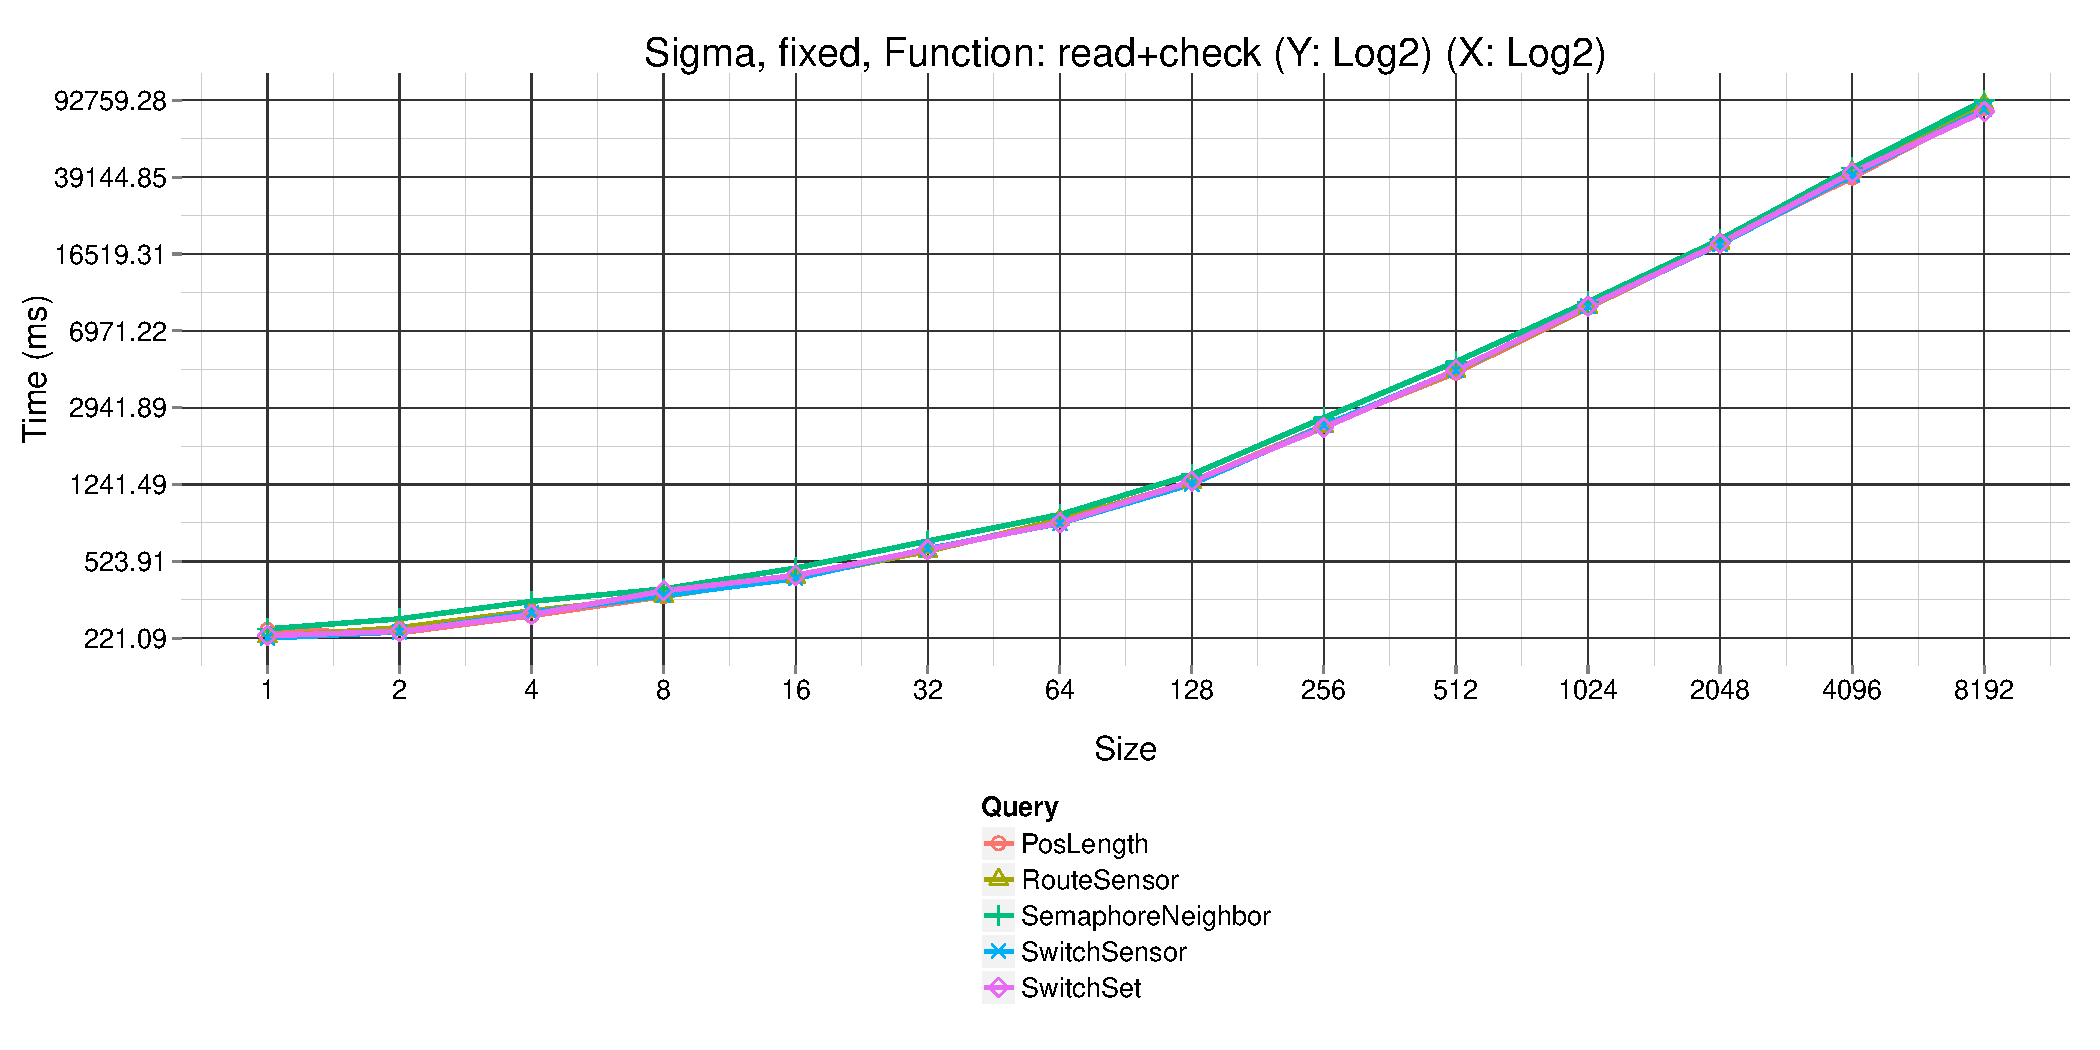
\includegraphics[width=\textwidth]{figures/fixed-Sigma-GroupBy-Query-time-batch-validation.pdf}
  \caption{\SIGMA fixed validation batch}
  \label{fig:SigmaFixedValidationBatch}
\end{figure}

\begin{figure}[h!tb]
  \centering
  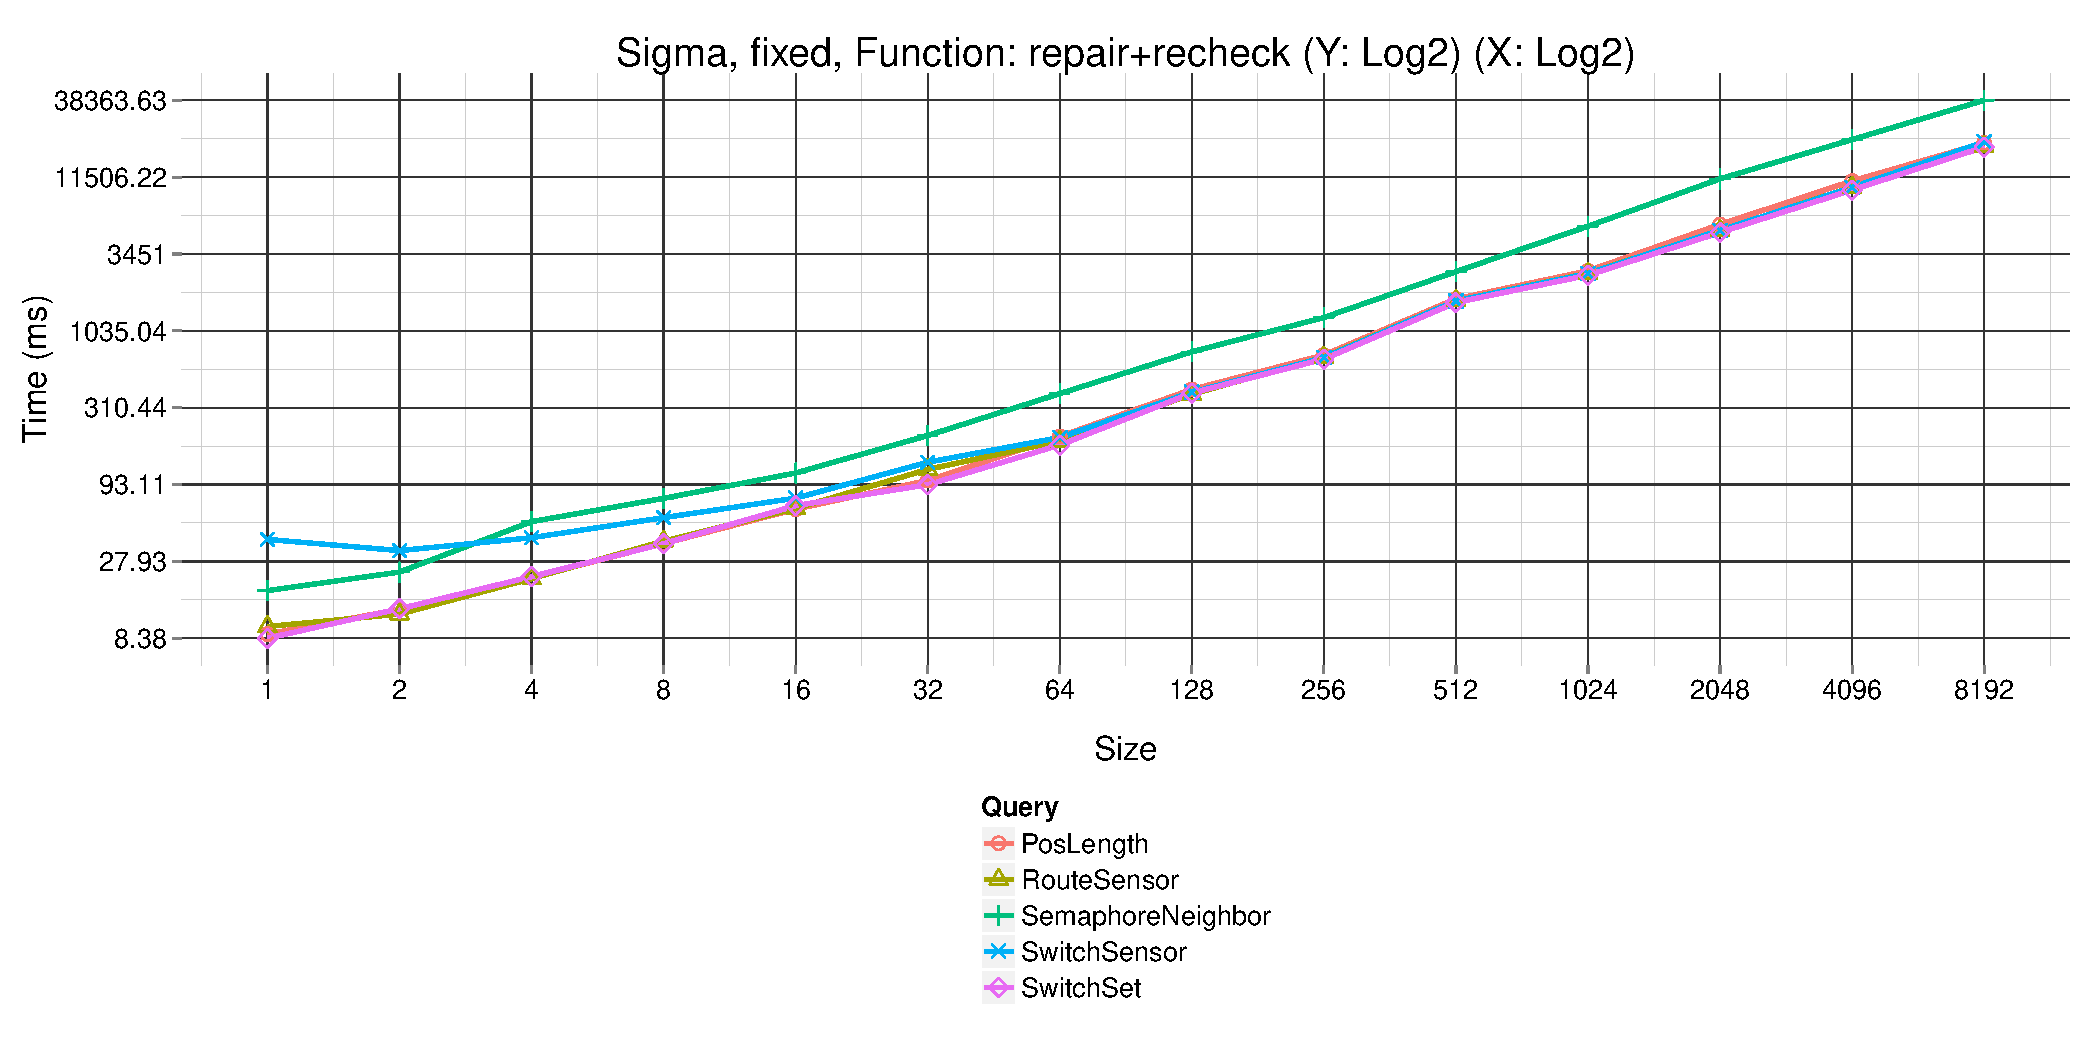
\includegraphics[width=\textwidth]{figures/fixed-Sigma-GroupBy-Query-time-revalidation.pdf}
  \caption{\SIGMA fixed revalidation}
  \label{fig:SigmaFixedReValidationBatch}
\end{figure}

\begin{figure}[h!tb]
  \centering
  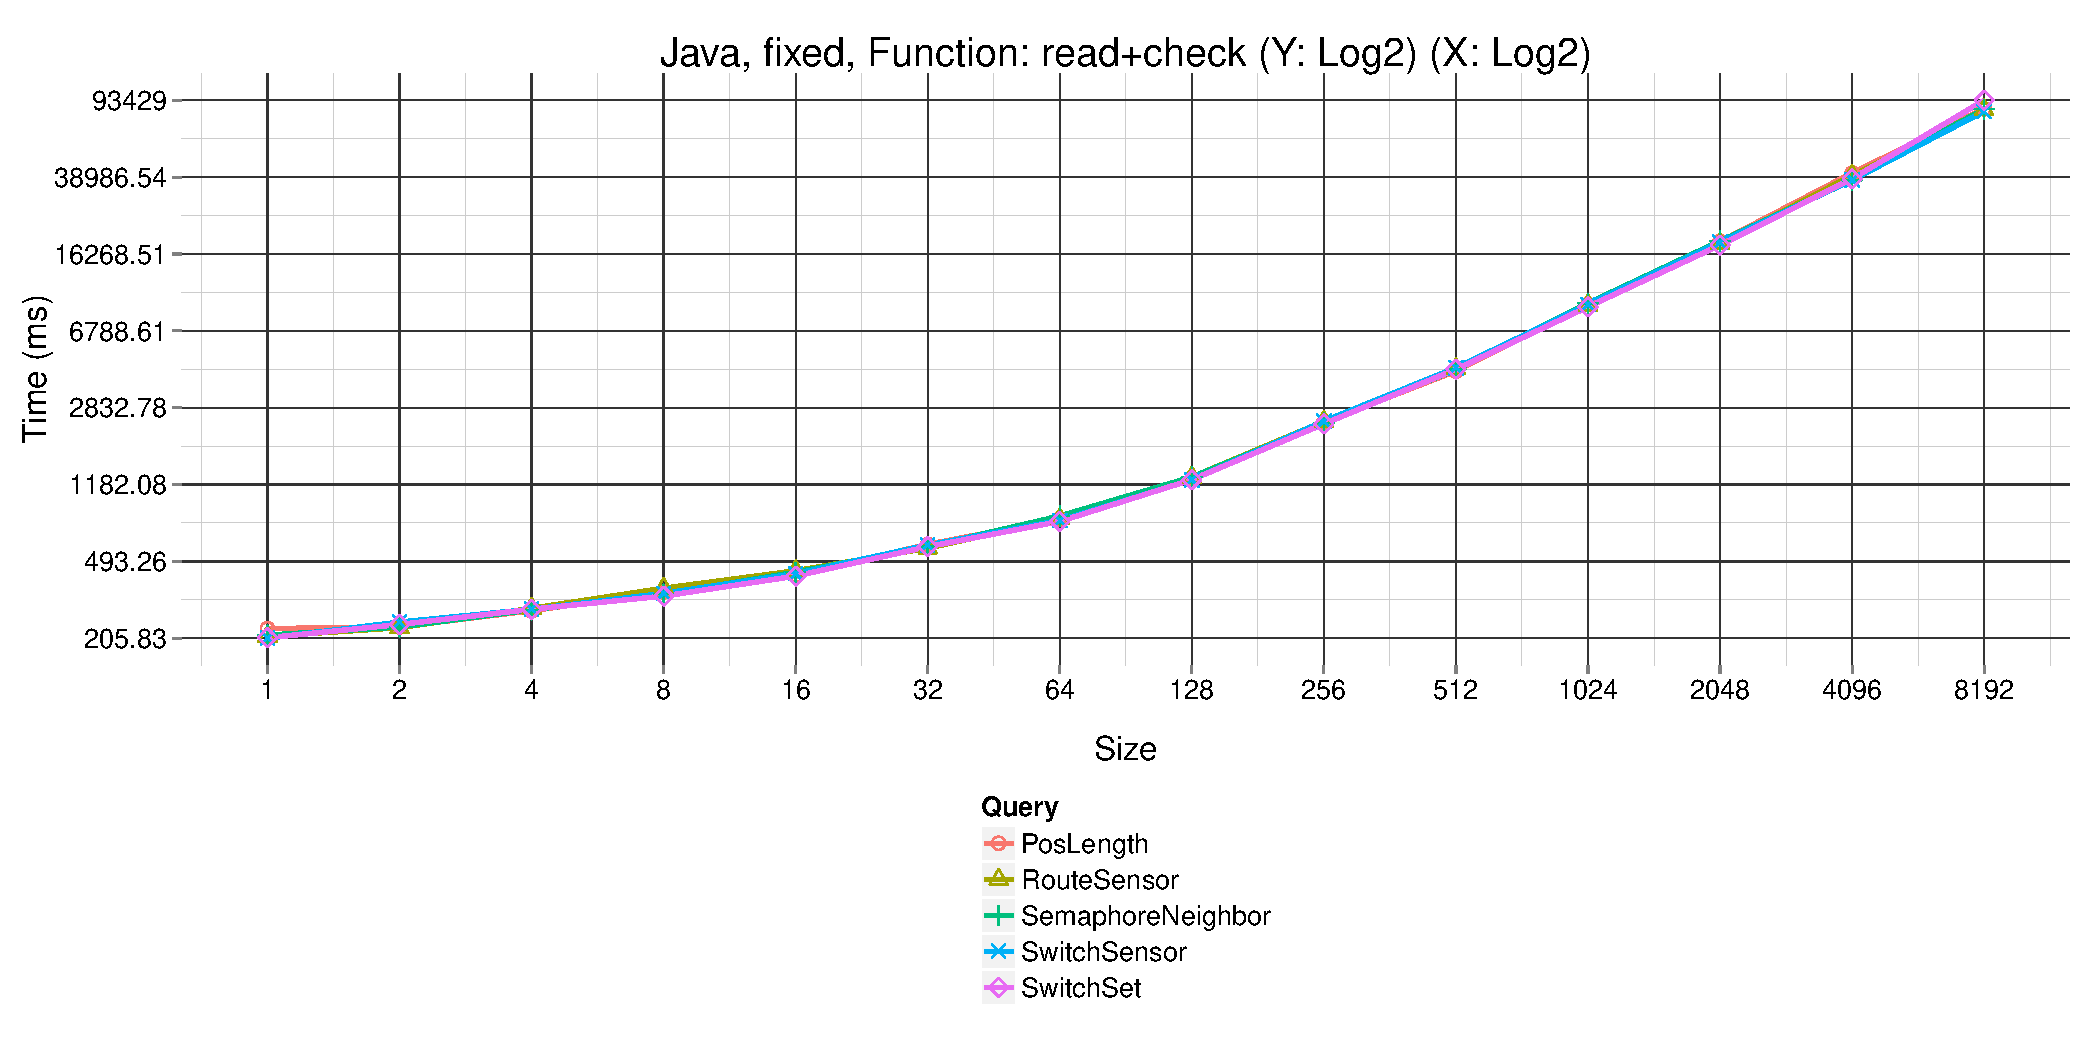
\includegraphics[width=\textwidth]{figures/fixed-Java-GroupBy-Query-time-batch-validation.pdf}
  \caption{Java fixed validation batch}
  \label{fig:JavaFixedValidationBatch}
\end{figure}

\begin{figure}[h!tb]
  \centering
  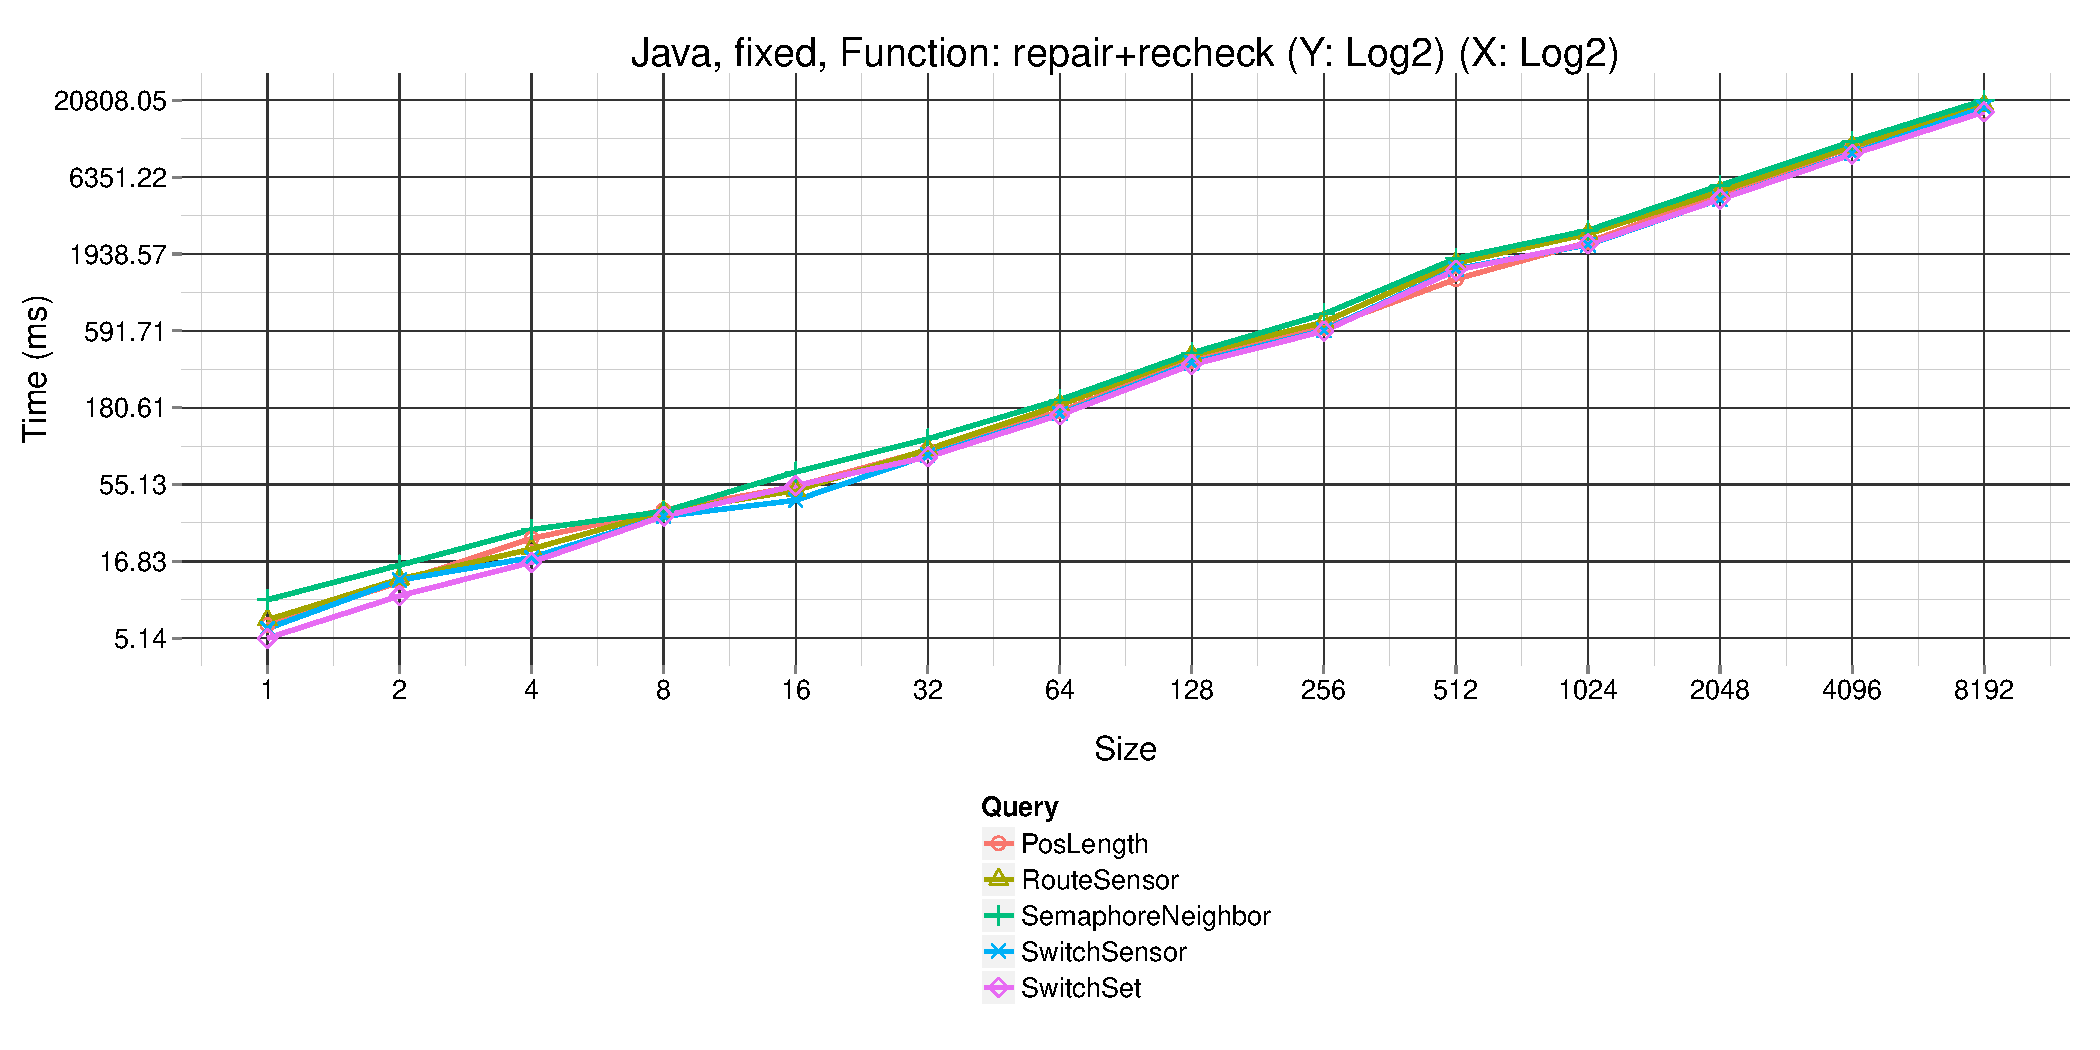
\includegraphics[width=\textwidth]{figures/fixed-Java-GroupBy-Query-time-revalidation.pdf}
  \caption{Java fixed revalidation}
  \label{fig:JavaFixedReValidationBatch}
\end{figure}

\clearpage
